\documentclass[11pt, a4paper, oneside]{book}

% Um sprache umzustellen
% \usepackage[ngerman]{babel}
\usepackage[english]{babel}

% Restliche Settings einfügen
\usepackage{Setup/settings}

% Einstellungen für Metainformation in PDF-Datei
\hypersetup{pdftitle={ESC241 Pion and Muon lifetime},
            pdfauthor={Till Böhringer, Lucien Käser, Marc Urech, Richard Salnikov}}

% Was im Footer stehen soll, ifoot -> links, cfoot -> mitte
\ifoot{Pion and muon lifetimes}
\cfoot{ESC241}

% Allgemeine weite um alle Figures darauf zu beziehen
\newcommand\Plotwidth{0.8}
\newcommand\DoublePlotwidth{0.9}
\newcommand\Bilderwidth{0.8}

% Setup wie siunix zahlen schreibt
\sisetup{group-separator = {'}, group-digits = integer}

% some stuff to make writing this report easiert
\newcommand{\electron}{$e^{-}$}
\newcommand{\pion}{$\pi^{-}$}
\newcommand{\muon}{$\mu^{-}$}

\lstset{language=python,
       basicstyle=\footnotesize\ttfamily,
  }

\usepackage{multirow}

\begin{document}

% Bitte Titlepage noch bearbeiten falls nötig
\newgeometry{bottom=1cm, top=4cm} % die Abstände von oben und unten korrigieren
\begin{titlepage}
    \setlength{\headheight}{0cm}
	%\centering
	\includegraphics[width=0.45\textwidth]{\thelogofilename}\par\vspace{1cm}
    % \includesvg[width=0.45\textwidth]{\thelogofilename}\par\vspace{1cm}
	
	\centering
	
	{\bfseries\LARGE University of Zurich\par}
	\vspace{0.7cm}
	
	{\Huge\bfseries Pion and muon lifetimes\par}
	\vspace{0.7cm}

	{\LARGE Data analysis 2025 \par Group project IV \par }
	\vfill

    {\large Authors:\par\vspace{0.2cm}}
	{\Large\itshape Till Böhringer\\ \href{mailto:tillnils.boehringer@uzh.ch}{tillnils.boehringer@uzh.ch} \par
	\Large\itshape Lucien Käser\\ \href{mailto:luciendarian.kaeser@uzh.ch}{luciendarian.kaeser@uzh.ch} \par
	\Large\itshape Marc Urech\\ \href{mailto:marcandre.urech@uzh.ch}{marcandre.urech@uzh.ch} \par
	\Large\itshape Richard Salnikov\\ \href{mailto:richardivan.salnikov@uzh.ch}{richardivan.salnikov@uzh.ch} \par}
	\vfill

	
	{\large Lecturer:\par\vspace{0.2cm}}
	{\Large Patrick Owen}
	\vfill
	\vfill

% Bottom of the page
	{\large \today\par}
\end{titlepage}
\restoregeometry % das das restliche Dokument wieder die normale Geometrie hat
\frontmatter

\tableofcontents
\mainmatter

\chapter{Abstract}
%Goal
The goal of this project is the estimate the mean lifetimes for negatively charged pions (\pion) and muons (\muon). 

%Method
Using the known decay law of the \pion-\muon-\electron chain, decay data is generated and analysed through a binned maximum likelihood fit as wel as a least squared method. The simulation is then validated using the pull. A more realisitic version of the simulation is also done, where each simulated decay time is seared with a previously defined value. This is done to take the finite time resolution of the experimental apparatus into account.

%Main Results
Results indicate, that the binned maximum likelihood fit, which was minimized using a combination of \lstinline{scipy.minimize} as well as a markov-chain-monte-carlo minimizer, returns the better estimations for the lifetimes in both simulations. 
%Conclusion

% Short summary: goal, method, main results, ... 

\chapter{Introduction}
% what we want to do
In this project, a simplified simulation of an experiment will be performed to measure the lifetimes of pions (\pion) and muons (\muon) charges.

% problem description
\section{Motivation}
Negatively charged pions (\pion) are composite particles that consist of a down quark and an up antiquark. They are unstable and decay predominantly to a muon (\muon) and a muon-antineutrino ($\bar{v_{\mu}}$). The muon, a heavier partner of the electron, is also unstable and decays into an electron (\electron), a muon-neutrino ($v_{\mu}$) and an electron antineutrino ($\bar{v_{e}}$). Neglecting any experimental effects, the time distribution of the \electron produced in the decay chain is given by

\begin{equation}
    N(t) = \frac{N_0}{\tau_{\mu} - \tau_{\pi}}  \left[ \exp{-\frac{t}{\tau_{\mu}}} - \exp{-\frac{t}{\tau_{\pi}}} \right]
    \label{eq:decay_chain_equation}
\end{equation}



Where $\tau_{\mu}$ and $\tau_{\pi}$ are the mean lifetimes of the \muon and \pion respectively. A measurement of this time distribution allows extracting times for $\tau_{\mu}$ and $\tau_{\pi}$.

\section{Setup}

The basic elements of the corresponding real experiment are shown in Figure \ref{fig:experimental_setup} negatively charged pion (\pion) is stopped in the third scintillator. The electron emitted (\electron) is then detected in the fifth scintillator. The time difference between the moment the \pion is stopped in the third scintillator and the \electron is detected in the fifth scintillator is recorded. A spectrum of time differences for many such events will allow for an estimation of the half life times of the \pion ($\tau_{\pi}$) and the \muon ($\tau_{\mu}$).

\begin{figure}[h]
\begin{center}
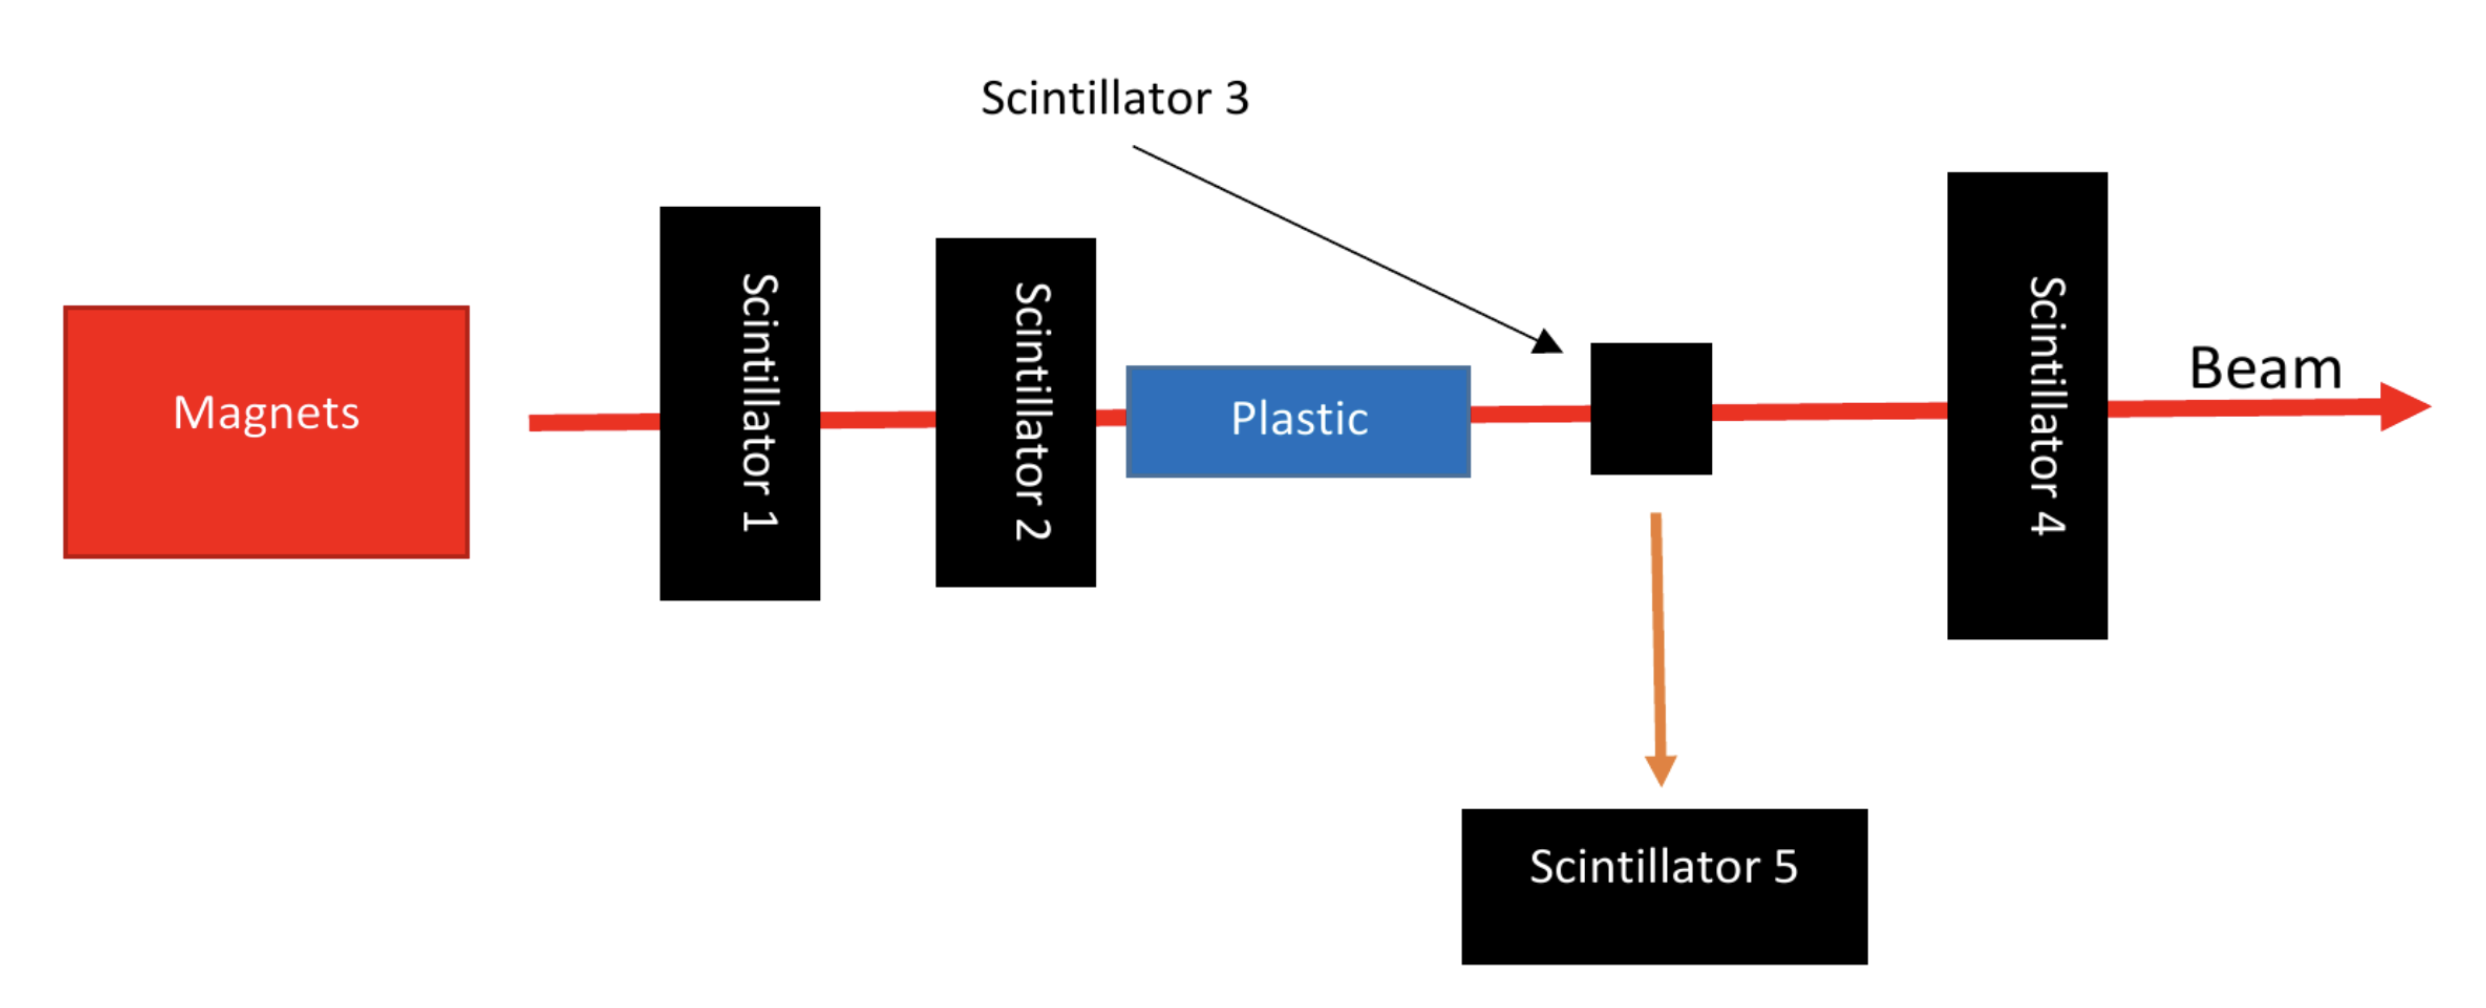
\includegraphics[width=0.7\textwidth]{images/experimental_setup.png}
\end{center}
\caption{Simplified sketch of the setup of the experiment (from the project documentation). A beam containing \pion passes through scintillators 1 and 2 and a piece of plastic to slow them down, such that they stop in scintillator 3. Scintillator 4 is a counter to reject events in which the beam particle was not stopped in scintillator 3. Electron \electron created in the decay chain are detected in scintillator 5. The signal from scintillator 3 starts a clock, the signal from scintillator 5 stops it.}
\label{fig:experimental_setup}
\end{figure}

\section{Validation of the simulation using the pull}
\begin{equation}
    \si{pull} = \frac{\bar{\tau} - \tau}{\sigma_{\bar{\tau}}}
    \label{eq:pull}
\end{equation}
The pull allows for a check of the estimated values. The pull of many simulations should follow a gaussian distribution with a mean of 0 as well as a standard deviation of 1. A deviation from these values can be an indication for the following problems:

Deviations in the mean value from 0, indicate a bias in the estimation of the lifetimes. Whereas a standard deviation larger or smaller than 1 indicate an under- / overestimation of the uncertainties. 

\section{Minimization of the likelihood}
The likelihood of a data set is given by the following equation:

\begin{equation}
    L = P(x | theta)
    \label{eq:likelihood_base}
\end{equation}

To simplify computation as well as numerical stability, the negative log likelihood is used. In the case of the decay times, the nll is given by:
\begin{equation}
  \log{nll} = -\sum_{i=1}^{N} c_i \cdot \log{\bar{c_i}} - \bar{c_i} - \log{c_i!}
  \label{eq:likelihood}
\end{equation}
where $c_i$ is the true number of counts in the bin $i$ and $\bar{c_i}$ the expected count.

\section{Computational implementation}
In this project, a simplified version of the experiment is simulated. At first, \num{10000} decay time measurements are simulated using the known values of the lifetimes of the \pion and \muon. This corresponds to the time difference between the moment the \pion is stopped in scintillator 3 and the \electron is detected in scintillator 5. Working with these simulated decay times, the goal is to extract the lifetimes of the \pion and \muon.

For the implementation python 3.10.11 is used, with the following packages:
\begin{itemize}
    \item numpy 2.0.0
    \item matplotlib 3.9.2
    \item scipy 1.14.1
    \item pandas 2.2.3
\end{itemize}
All used packages are freely available under an open-source license. 
The full implementation of the simulation as well as this documentation is available on \cite{GitHub}.

% goal of the simulation
% short theoretical background

\FloatBarrier
\chapter{Methods}
In this chapter, the two performed simulations are described. The first one is an estimation of the lifetimes of the \pion and \muon using previously generated decay times. The second simulation will build on the first one, but will include the finite time resolution of the apparatus. 

\section{Simple simulation} \label{sec:simple_simulation}
The goal of the first simulation is to simulate the decay of \pion and \muon without taking the finite time resolution of the apparatus into account. The simulation for this will take the following steps:
\begin{itemize}
  \item Generation of \num{10000} decay times using equation \ref{eq:decay_chain_equation} with the known    values of the lifetimes.
  \item Estimation of the lifetimes including their respective uncertainties using a binned maximum likelihood fit to the histogram of the decay times.
  \item Repeat the simulation \num{100} times to get a distribution of the estimates and the pulls.
  \item Validation of the simulation using the pull, as defined in equation \ref{eq:pull}.
\end{itemize}

\section{A bit more realistic simulation} \label{sec:realistic_simulation}
In section \ref{sec:simple_simulation}, the distribution of points were directly generated from the distribution \ref{eq:decay_chain_equation}. This isn't realistic, since the measurements itself aren't precise and have some noise to them. To implement this into the simulation, all simulated decay times got "smeared" by a random value drawn from a normal distribution. The standard deviation of this distribution was set to three different values 0.01, 0.1, 1 times the \pion Mean lifetime. The resulting histogram can be seen in figure \ref{fig:smeared_hist}.

This more accurate simulation will be done in the following steps:
\begin{itemize}
  \item Generation of \num{10000} decay times using equation \ref{eq:decay_chain_equation} using the know values of the lifetimes. A "smear" will be done on each decay time with a random offset drawn from a gaussian distribution with a mean of $\mu = 0$ and a standard deviation $\sigma_t$. This will be done for the following values of $\sigma_t = \frac{1}{100}, \frac{1}{10}, 1 * \tau$
  \item The now more realistic data is now piped through the same algorithms as in section \ref{sec:simple_simulation}. Here both the MLM as well as the LSM are used.
  \item The results of the more accurate simulation can then be compared to see if and how the smearing influences the fitting of the lifetimes.
\end{itemize}


\chapter{Results}
% present key results (plots, tables, values)
% explain findings objectively, without interpretation

In this chapter, the results of the simulations including their implementations are discussed.

\section{Implementation of the simple simulation} \label{sec:simple_simulation_results}

\subsection{Simulation of the decay times}
To generate the \num{10000} decay times, equation \ref{eq:decay_chain_equation} is used, with the known values of the lifetimes of the \pion and \muon. The known values are given by: \cite{ParticleDataGroup:2024cfk}

\pion Mean lifetime: \qty{2.6033(0.0005)e-8}{\s} \\
\muon Mean lifetime: \qty{2.1969811(0.0000022)e-6}{\s} \\

%TODO: add a plot of the distribution without anything in it
The decay times are generated using the accept-reject method. For this, a random point on the domain of the distribution is generated (t, y). If the generated point is below the distribution, it is accepted, if not, it is rejected. This is done until the target number of points is reached. 
The decay time $t$ is generated using a uniform distribution between 0 and \qty{1}{\s}. The count $y$ is also drawn from a uniform distribution between \qty{0} and the maximum value of the target distribution $max(N(t))$

The random points generated are shown in figure \ref{fig:histogram} in form of a histogram. The overlaid distribution is given by equation \ref{eq:decay_chain_equation} using the known lifetimes.


\begin{figure}[H]
    \centering
    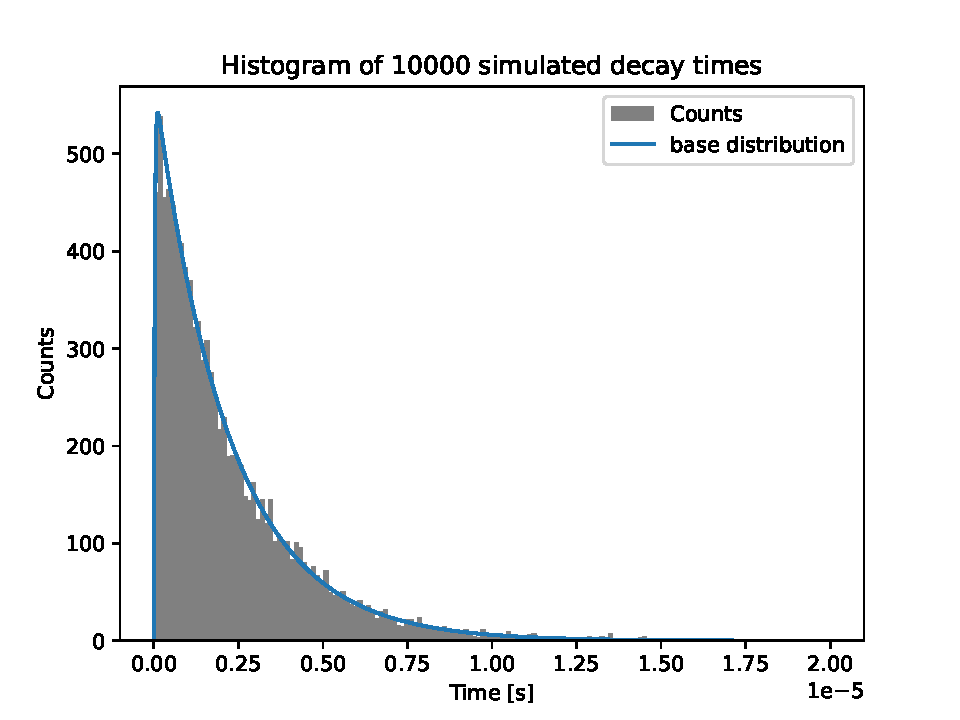
\includegraphics[width=\Plotwidth\textwidth]{images/simulated_decay_histogram_150bins.pdf}
    \caption{The histogram generated using accept-reject method.}
    \label{fig:histogram}
\end{figure}

\subsection{Estimation of the lifetimes}
Next a binned-maximum-likelihood\footnote{From this point on the abreviation MLM will be used to reference the binned-maximum-likelihood method} (MLM) was performed on the histogram. For this the likelihood was calculated according to equation \ref{eq:likelihood} and minimized using the combination of scipy's minimization function as well as a custim markov-chain-monte-carlo (mcmc) minimizer. Although this method worked, it presented with multiple problems: The entire estimation process took a long time, as the mcmc-method required to run for some \num{10000} iterations to get a good estimate. The results of the estimation can be seen in figure \ref{fig:likelihood_results}.

\begin{figure}[H]
    \centering
    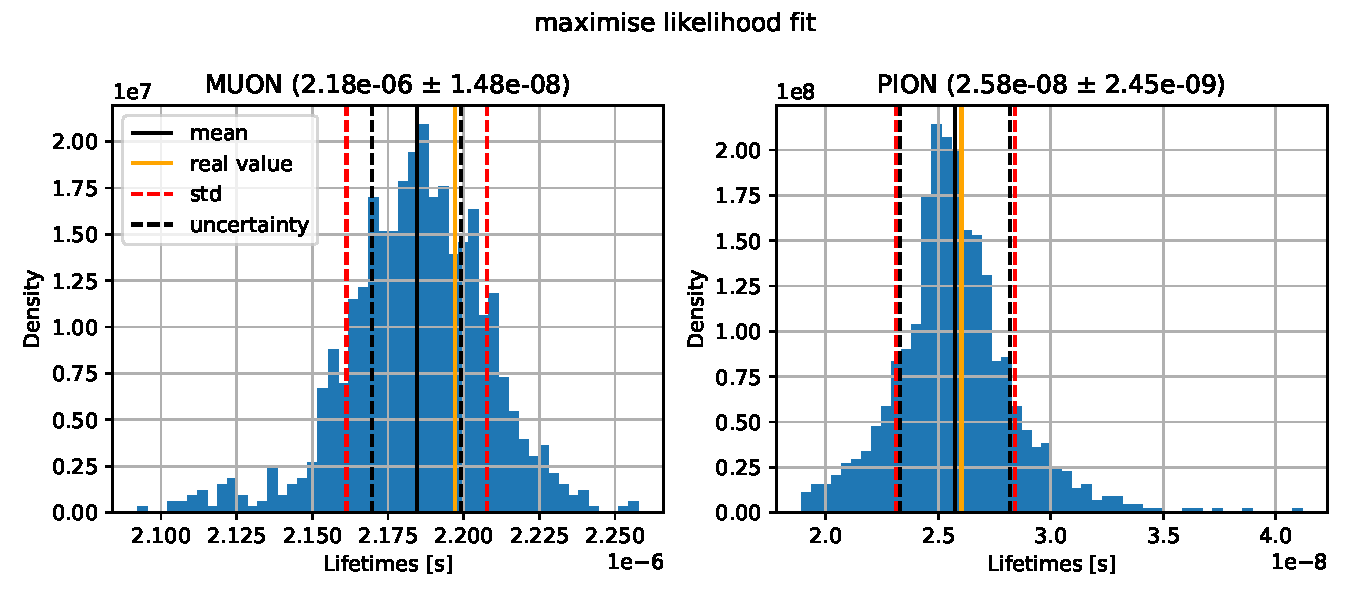
\includegraphics[width=\DoublePlotwidth\textwidth]{images/estimators_hist_likelihood.pdf}
    \caption{Estimation of the lifetimes using the binned maximum likelihood method}
    \label{fig:likelihood_results}
\end{figure}

To improve the efficiency of the estimation, the least squared method\footnote{From this point on the abreviation LSM will be used to reference the least-squares method} (LSM) was also considered. Using the same data, it returned better estimations for the lower end of the decay time spectrum as can be seen in equation \ref{fig:comparison_estimators}. The LSM method was implemented using the \lstinline|curve_fit| function from the scipy package. The results of the estimation can be seen in figure \ref{fig:least_squares_results}.

\begin{figure}[H]
    \centering
    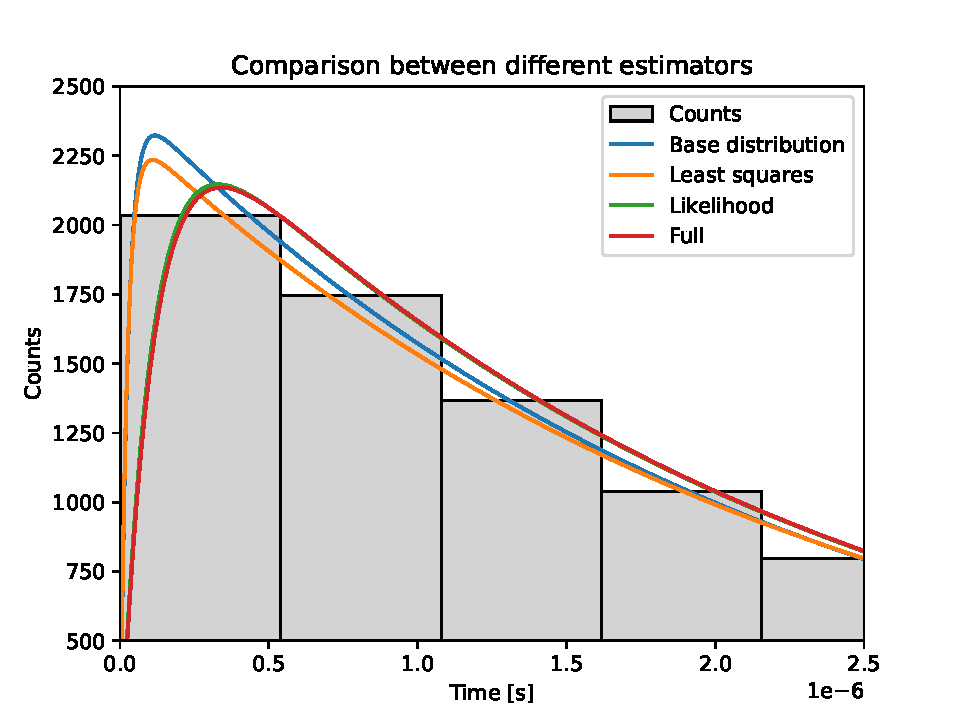
\includegraphics[width=\Plotwidth\textwidth]{images/comparison_estimators.pdf}
    \caption{Comparison between different estimators and the base distribution, overlaid on the histogram.}
    \label{fig:comparison_estimators}
\end{figure}

\begin{figure}[H]
  \centering
  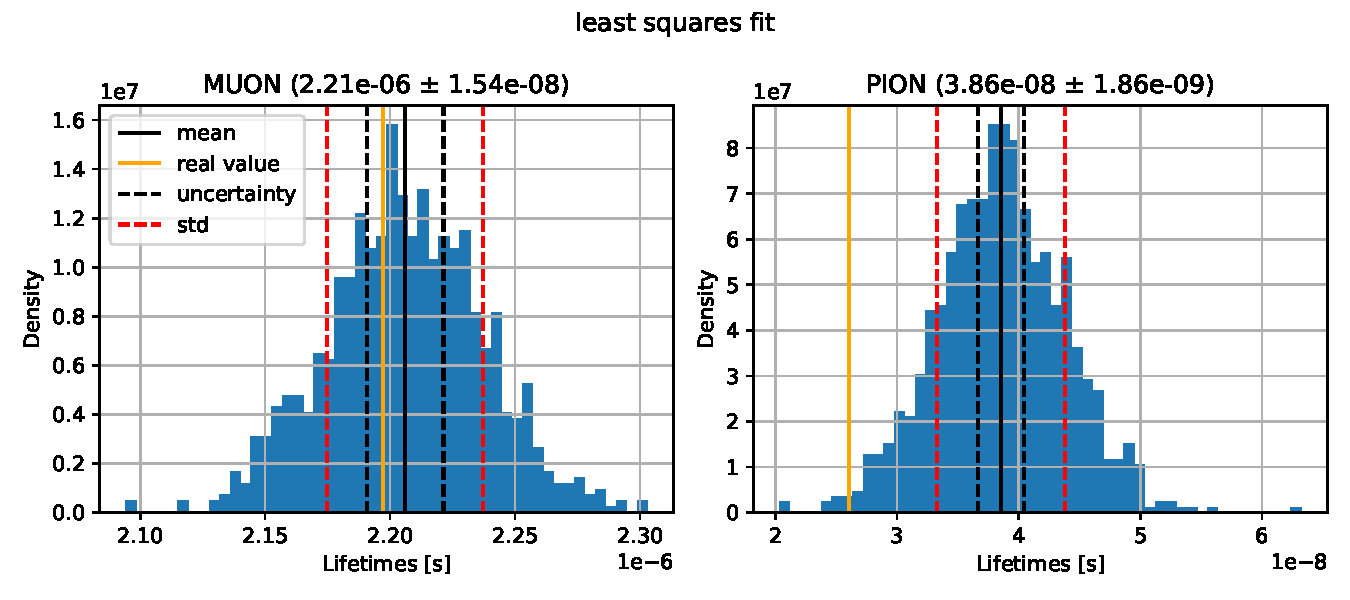
\includegraphics[width=\DoublePlotwidth\textwidth]{images/estimators_hist_least_squares.pdf}
  \caption{Estimation of the lifetimes using the binned maximum likelihood method}

  \label{fig:least_squares_results}
\end{figure}


\subsection{Uncertainties of the estimators}
For the estimation of the uncertainties, two different methods were used. 
\begin{itemize}
    \item For the MLM, the uncertainties were calculated by finding the points, where the likelihood is \qty{0.5} (absolute) away from the minimum. This is done by using the minimal value of the likelihood and subtracting \qty{0.5} from it. Then the roots of the likelihood are calculated using the newton-raphson method. 
    \item For the LSM, the uncertainties were calculated using the covariance matrix, which is returned as part of the \lstinline{minimization_results} object. The uncertainties are given by the root of half of the diagonal elements of the covariance matrix.
\end{itemize}

To check if the estimations as well as the uncertainties are correct, the pull was calculated using equation \ref{eq:pull}. According to the definition, the pull should be a normal distribution with a mean $\mu$ of 0 and a standard deviation $\sigma = 1$. The results of the pull can be seen in figure \ref{fig:pull_likelihood_method} for the MLM method and in figure \ref{fig:pull_least_squares_method} for the LSM. 

\begin{figure}[H]
  \centering
  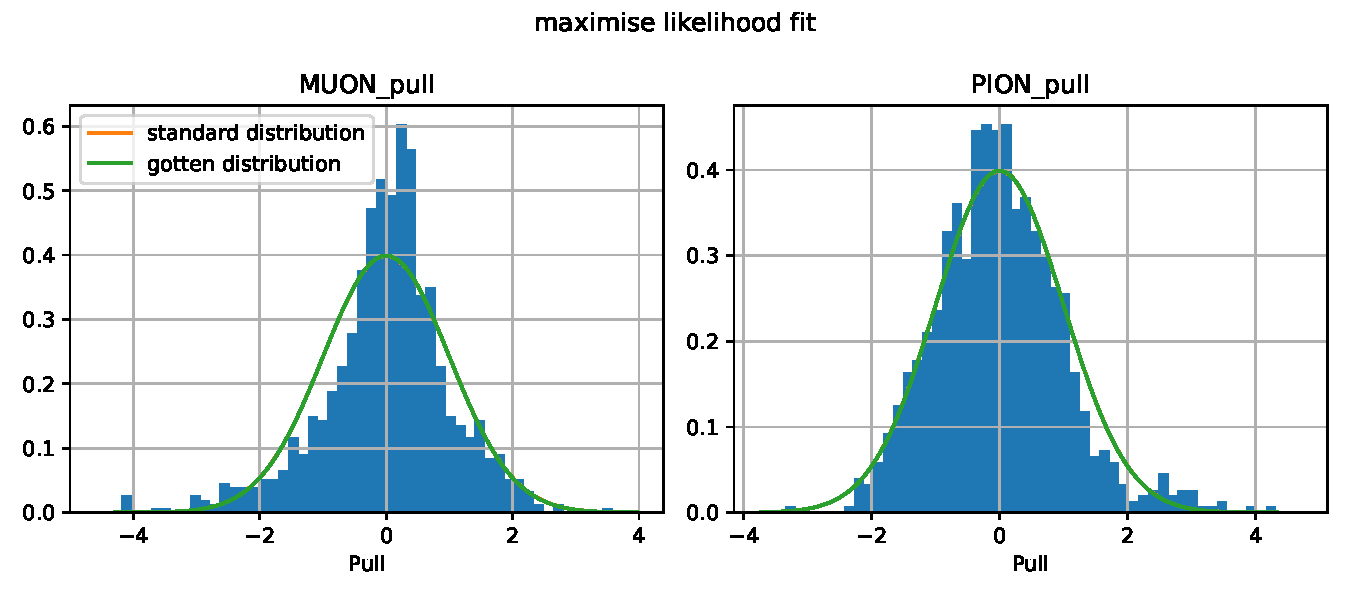
\includegraphics[width=\DoublePlotwidth\textwidth]{images/estimators_pull_likelihood.pdf}
  \caption{Pull of the estimations using the binned maximum likelihood method.}
  \label{fig:pull_likelihood_method}
\end{figure}

\begin{figure}[H]
  \centering
  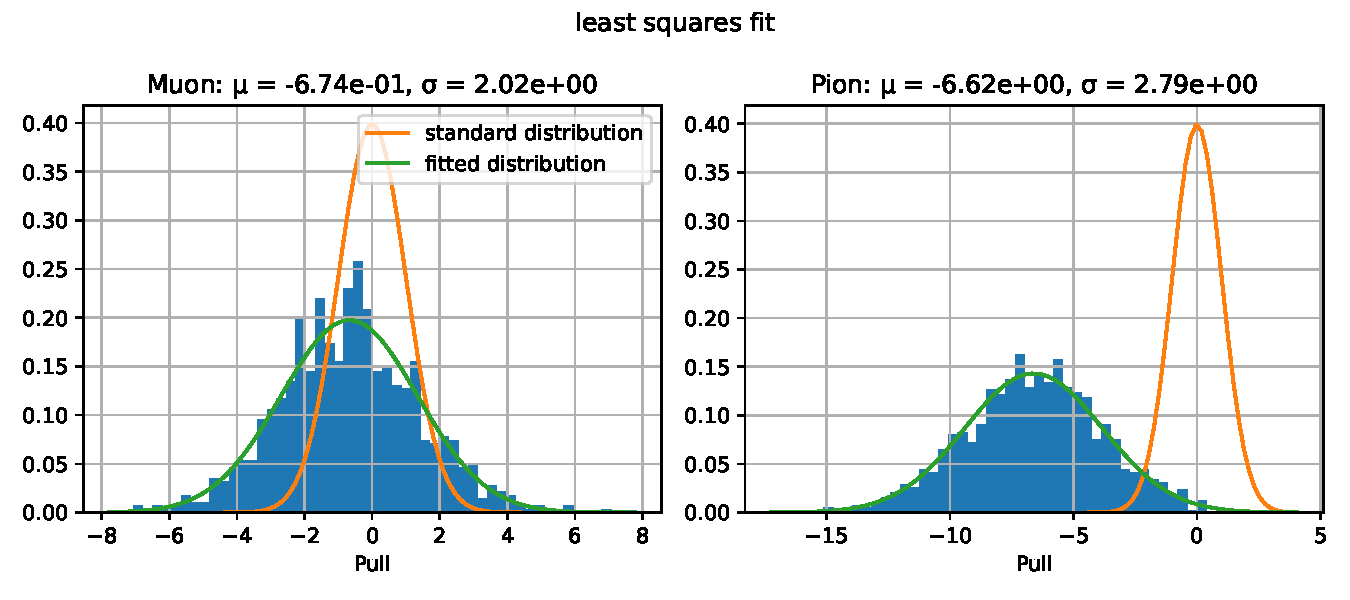
\includegraphics[width=\DoublePlotwidth\textwidth]{images/estimators_pull_least_squares.pdf}
  \caption{Pull of the estimations using the least squares method.}
  \label{fig:pull_least_squares_method}
\end{figure}

\section{Comparison of the estimations and evaluation of the pull}
Using the two different methods, the lifetimes of the \pion and \muon were estimated. The results are shown in table \ref{tab:results}.

\subsection{Results of the estimations}

\begin{table}[H]
  \begin{tabular}{l|ccc}
                & true value & MLM & LSM \\ \hline
  muon lifetime & $2.1969811(22)*10^{-6}\si{s}$ & $2.184(15)*10^{-6}\si{s}$ & $2.207(15)*10^{-6}\si{s}$ \\
  pion lifetime & $2.6033(5)*10^{-8}\si{s}$ & $2.581(246)*10^{-8}\si{s}$ & $3.836(186)*10^{-8}\si{s}$                    
  \end{tabular}
  \caption{Results of the estimations of the lifetimes using both the MLM as well as the LSM. The true values are given by \cite{ParticleDataGroup:2024cfk}.}
  \label{tab:results}
\end{table}

As shown in Table \ref{tab:results}, the MLM produces values closer to the true lifetimes for both the \pion and \muon. Although the LSM is considerably faster, it fails to provide a good estimate for the \pion lifetime, even when uncertainties are accounted for.


%% -> This can be now found in the conclusion
%As can be seen in table \ref{tab:results}, the MLM results in better values, which are closer to the true values. Although the LSM is faster, it does not give a good result for the estimation of the \pion lifetime, as the value is way off even when taking the uncertainties into account.

% \begin{table}[H]
%   \begin{tabular}{l|ccc}
%                 & true value & binned-maximum-likelihood method & least-squares method \\ \hline
%   muon lifetime & $2.1969811(22)*10^{-6}\si{s}$ & $2.184(15)*10^{-6}\si{s}$ & $2.207(15)*10^{-6}\si{s}$ \\
%   pion lifetime & $2.6033(5)*10^{-8}\si{s}$ & $2.581(246)*10^{-8}\si{s}$ & $3.836(186)*10^{-8}\si{s}$                    
%   \end{tabular}
%   \caption{Results of the estimations of the lifetimes using both the binned-maximum-likelihood as well as the least-squares method. The true values are given by \cite{ParticleDataGroup:2024cfk}.}
%   \label{tab:results}
% \end{table}

%\begin{table}[H]
  %\begin{tabular}{lll}
  %                                      & MLM & LSM \\ \hline
  %\multicolumn{1}{l|}{Muon (mean, std)} & $\mu = 0.84$, $\sigma = 1.54 $             & $\mu = -0.67$, $\sigma %= 2.02$  \\
  %\multicolumn{1}{l|}{Pion (mean, std)} & $\mu = 0.163$, $\sigma = 1.04$            & $\mu = -6.62$, $\sigma% = 2.79$ 
%  \end{tabular}
%\end{table}

\subsection{Results of the pull} 

Using the pull, the results of the estimations can be evaluated. For any bias as well as the accuracy of the uncertainties as well. The results of the pull as shown in figure \ref{fig:pull_likelihood_method} and \ref{fig:pull_least_squares_method} are summarized in table \ref{tab:pull_results}\footnote{Uncertainties are represented in the following way: $a(b)$ which is to be understood as $a \pm b$. E.g: $1.23(50)*10^-5$ corresponds to $1.23*10^{-5} \pm 0.50 * 10^{-5}$}.

% \begin{table}[H]
%   \begin{tabular}{lll}
%                                         & bined-maximum-likelihood method & least-squares method \\ \hline
%   \multicolumn{1}{l|}{Muon (mean, std)} & $\mu = 0.84$, $\sigma = 1.54 $             & $\mu = -0.67$, $\sigma = 2.02$  \\
%   \multicolumn{1}{l|}{Pion (mean, std)} & $\mu = 0.163$, $\sigma = 1.04$            & $\mu = -6.62$, $\sigma = 2.79$ 
%   \end{tabular}
%   \caption{Comparison of the pull for the two methods}
%   \label{tab:pull_results}
% \end{table}

\begin{table}[H]
\centering
  \caption{Comparison of the pull for the two methods}
  \label{tab:pull_results}
  \begin{tabular}{l|ll}
                   & MLM                                & LSM \\ \hline
  Muon (mean, std) & $\mu = 0.84$, $\sigma = 1.54 $     & $\mu = -0.67$, $\sigma = 2.02$  \\
  Pion (mean, std) & $\mu = 0.163$, $\sigma = 1.04$     & $\mu = -6.62$, $\sigma = 2.79$ 
  \end{tabular}
\end{table}

The pull analysis (Table \ref{tab:pull_results}) further suggests that the MLM is the better method for this simulation, as the pulls for both lifetimes are close to the ideal value of 0. The standard deviations of $1.5$ for the \muon and $1$ for the \pion also indicate that the uncertainties are quite accurate. However, it is important to note that there is a slight bias in the \muon estimation, which directly affects the uncertainties and, consequently, the standard deviation of the pull.

% -> this can also be found in the conclusion
%As clearly visible in table \ref{tab:pull_results}, the MLM produces better estimations, as the mean of the pull for both the \muon and \pion lifetimes are closer to 0 and the standard deviation beeing closer to 1. The LSM on the other hand produces an good value for the estimation of the \muon lifetime, but a very bad one for the \pion lifetime. The mean of $\mu = -6.62$ indicates a very strong bias in the estimation and the standard deviation of $\sigma = 2.79$ indicates a very strong miscalculation in the uncertainties. 

\newpage
\section{A bit more realistic simulation} \label{sec:more_realisitic_results}

In section \ref{sec:realistic_simulation} the generated data got more realistic with differently strong smearing.

\subsection{Smeared with 0.01 times the \texorpdfstring{\pion}{pion} Mean lifetime}

In figure \ref{fig:results_smeared_0} is clear that the MLM yields better results as the LSF. Especially for the \pion lifetime the MLM gives an impressively precise result in terms of the mean that is close to the real\footnote{Real in terms of: "This is the value that the distribution is based on", not as in "The real \pion lifetime." The real lifetime is unknown and for calculating the distribution a result of a measurement was used.} value. Also, the uncertainties on the measurement are similar to the standard deviation, which means that the uncertainties get calculated correctly. This is also seen in figure \ref{fig:smeared_pull_0} which depicts the pull.

\begin{figure}[h]
\begin{subfigure}{\textwidth}
  \centering
  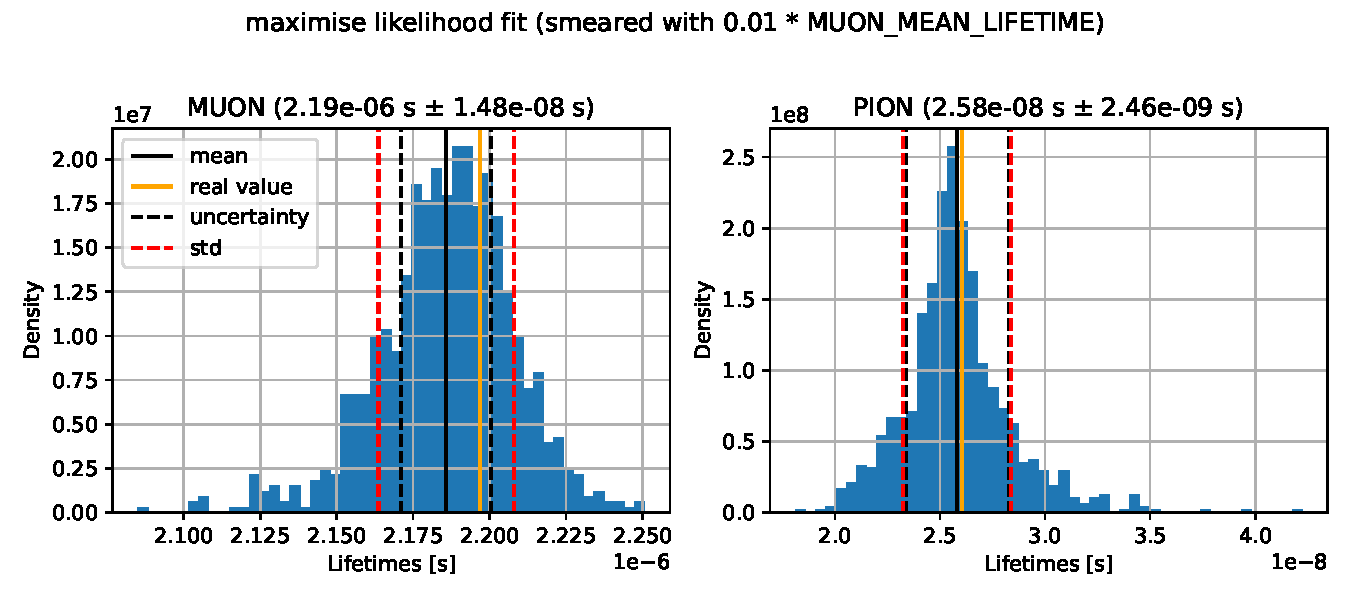
\includegraphics[width=\DoublePlotwidth\textwidth]{images/4b_hist_0_likelihood.pdf}
%   \caption{}
\end{subfigure}

\begin{subfigure}{\textwidth}
  \centering
  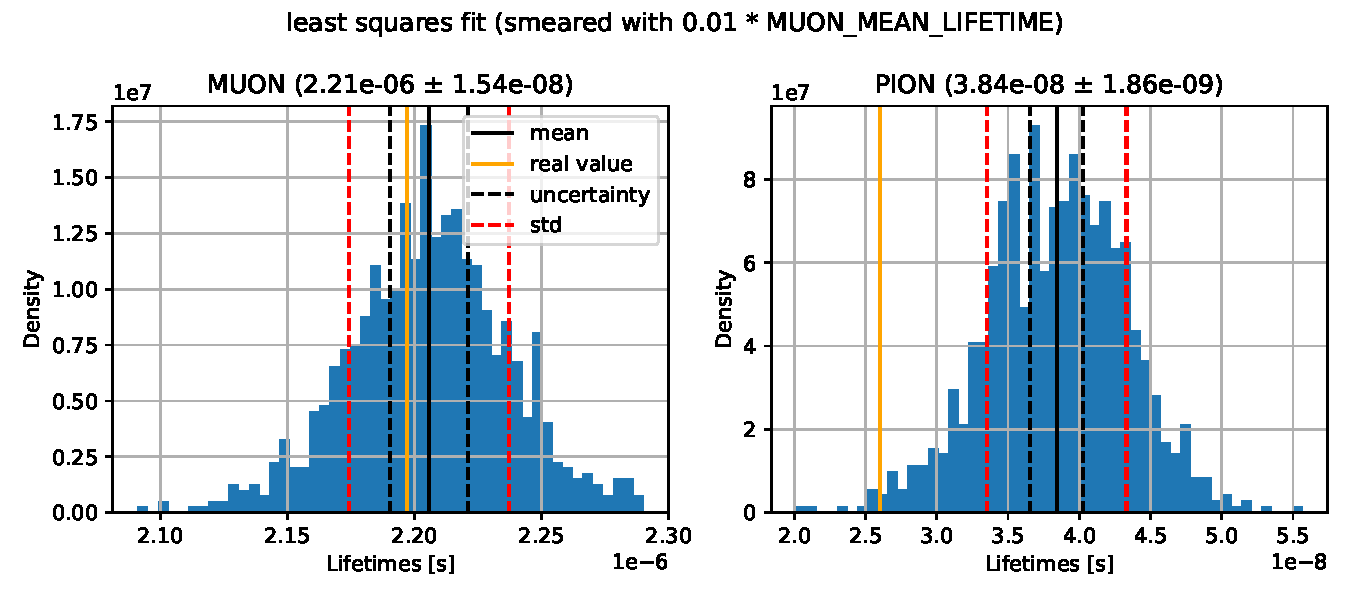
\includegraphics[width=\DoublePlotwidth\textwidth]{images/4b_hist_0_squares.pdf}
%   \caption{}
\end{subfigure}
\caption{Results of 1000 different sets of simulated and fitted data. Here the data was smeared with 0.01 time the \pion Mean lifetime.}
\label{fig:results_smeared_0}
\end{figure}

\begin{figure}[h]
    \centering
    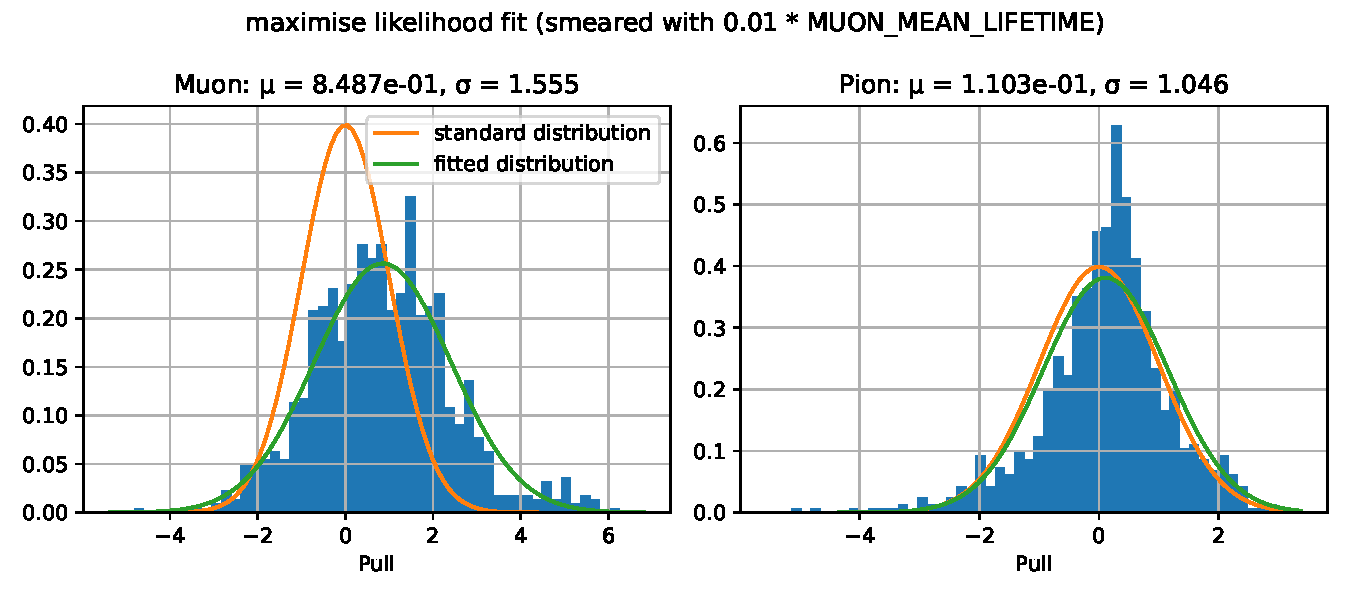
\includegraphics[width=\DoublePlotwidth\textwidth]{images/4b_pull_0_likelihood.pdf}
    \caption{The Pull of the result of the MLM from figure \ref{fig:results_smeared_0}. The pull shows how good the \pion lifetime fit is, because the fitted normal distribution is very similar to the standard normal distribution.}
    \label{fig:smeared_pull_0}
\end{figure}

\FloatBarrier
\subsection{Smeared with 0.1 times the \texorpdfstring{\pion}{pion} Mean lifetime}

Also, with bigger smearing the MLM gives better results, this is shown in figure \ref{fig:results_smeared_1}. In comparison to the less smeared results, the differences between uncertainties and standard deviations got bigger and the bias, the difference between the mean and the real value, also got bigger. In particular with the MLM, both means lie within the calculated uncertainties, which is not the case with the \pion lifetime from the LSM.

\begin{figure}[h]
\begin{subfigure}{\textwidth}
  \centering
  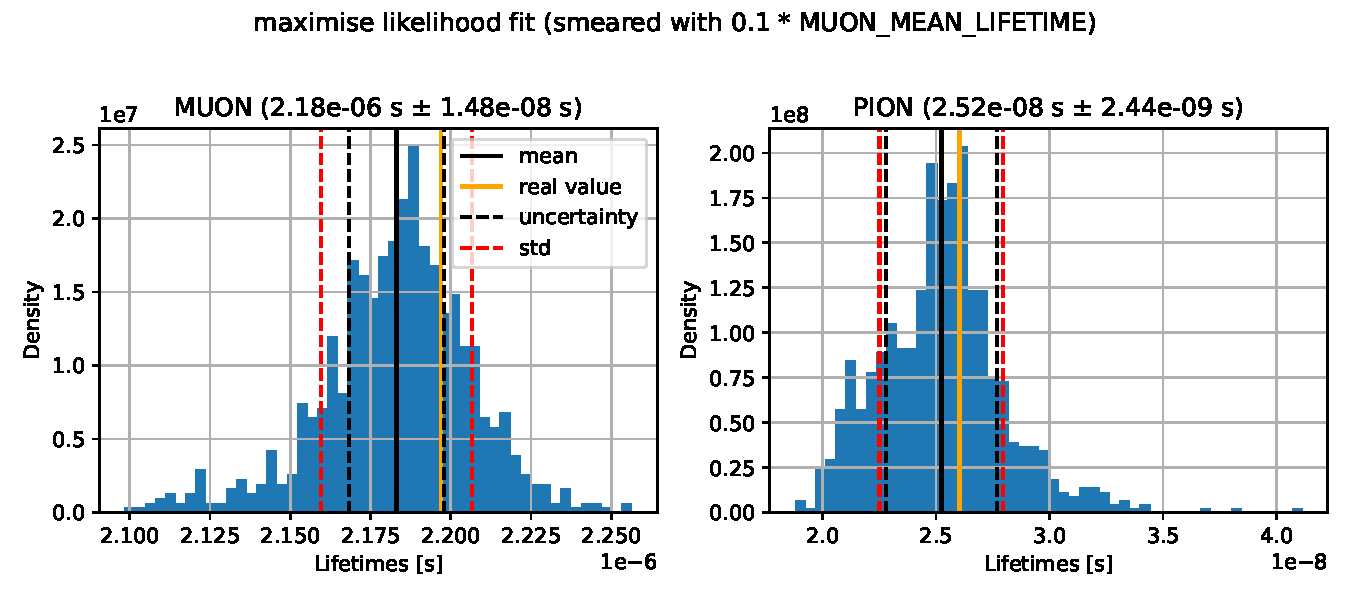
\includegraphics[width=\DoublePlotwidth\textwidth]{images/4b_hist_1_likelihood.pdf}
%   \caption{}
\end{subfigure}

\begin{subfigure}{\textwidth}
  \centering
  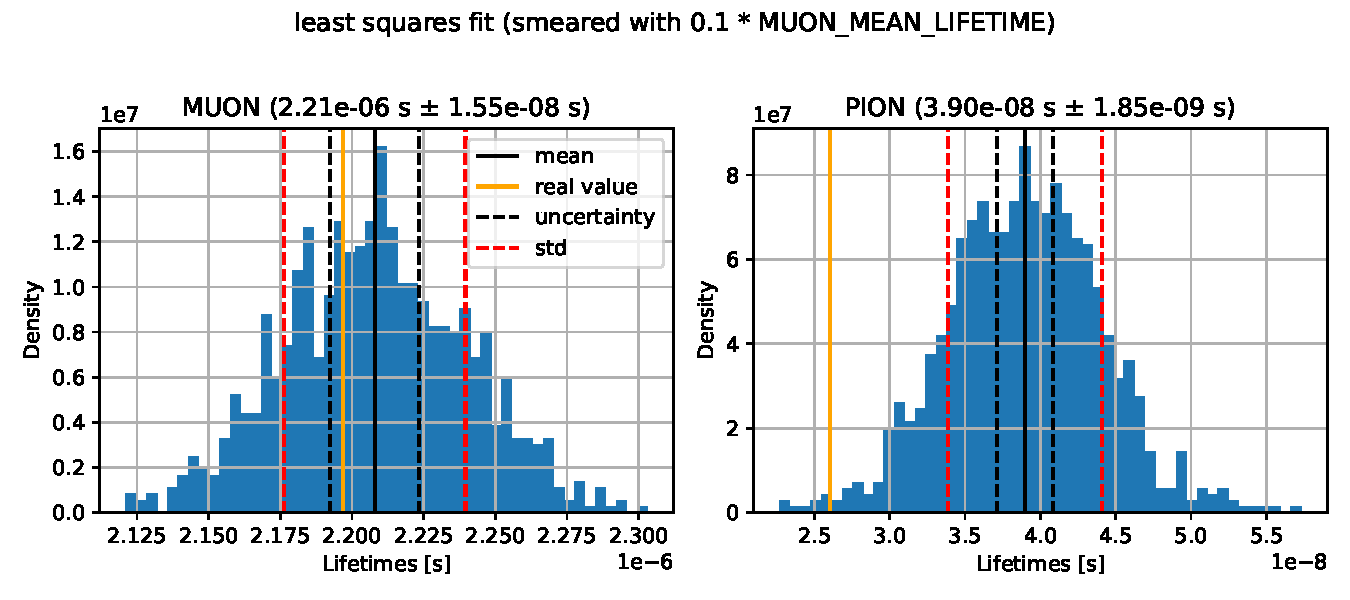
\includegraphics[width=\DoublePlotwidth\textwidth]{images/4b_hist_1_squares.pdf}
%   \caption{}
\end{subfigure}
\caption{Results of 1000 different sets of simulated and fitted data. Here the data was smeared with 0.1 time the \pion Mean lifetime.}
\label{fig:results_smeared_1}
\end{figure}

\FloatBarrier
\subsection{Smeared with 1 times the \texorpdfstring{\pion}{pion} Mean lifetime}

If the smearing gets to big, there start be be some problem with the MLM. The problem is that the fitting does not converge, and it just returns the initial guess. The possibility stands that with further tweaking of the parameters that get fed into the \lstinline{minimize} function, it will converge, but the initial guess is already close to the real values and there parameter are also bounded, so they can not wander to far away. If the setup of the fitting requires that the result is already known beforehand, the fitting itself becomes obsolete. In turn the SLM still gives results. The \muon lifetime is even close to the real value as with the more smeared data and the \pion lifetime gives a result. There is a significant bias to the \pion lifetime and the uncertainties get strongly underestimated, when they are compared to the standard deviation, but there is a result in the correct magnitude.

The situation with the MLM not converging could also be helped by changing the minimize-algorithm completely. In SciPy itself there is also the \lstinline{dual_annealing} option or even a full custom minimizer could be written like based for example on a Markov-Chain. This route would need more time and resources, but could be worth it, if the resulting algorithm would be implemented in a larger scale or even just multiple times.

\begin{figure}[h]
\begin{subfigure}{\textwidth}
  \centering
  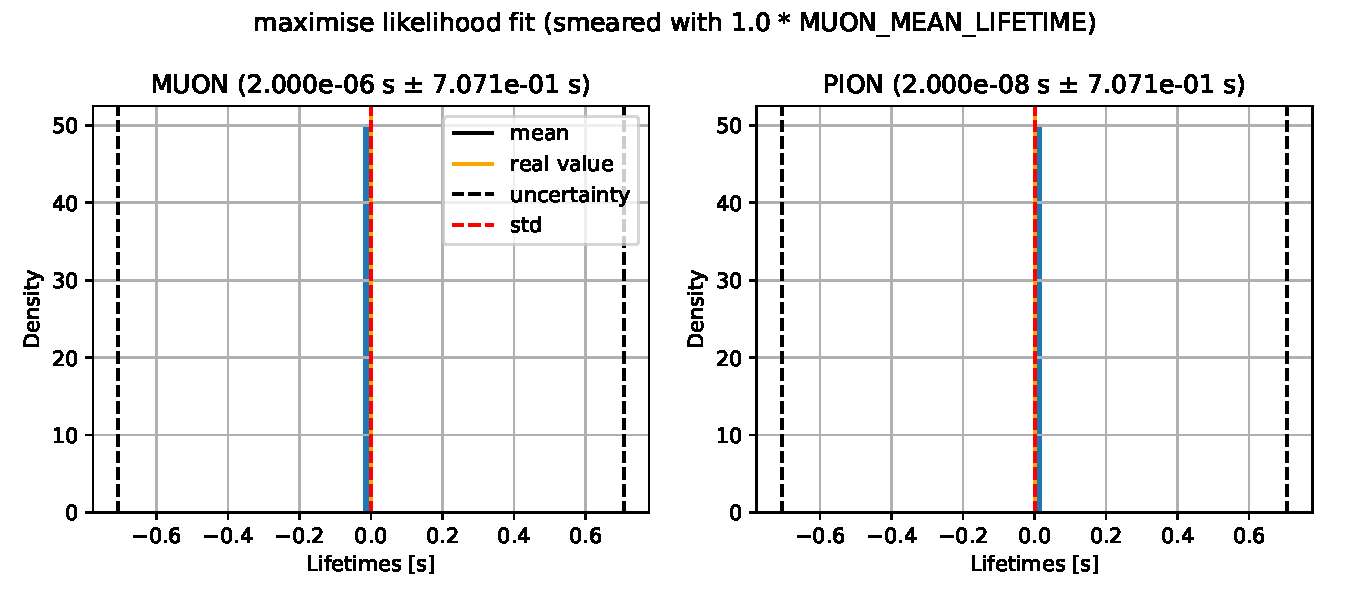
\includegraphics[width=\DoublePlotwidth\textwidth]{images/4b_hist_2_likelihood.pdf}
%   \caption{}
\end{subfigure}

\begin{subfigure}{\textwidth}
  \centering
  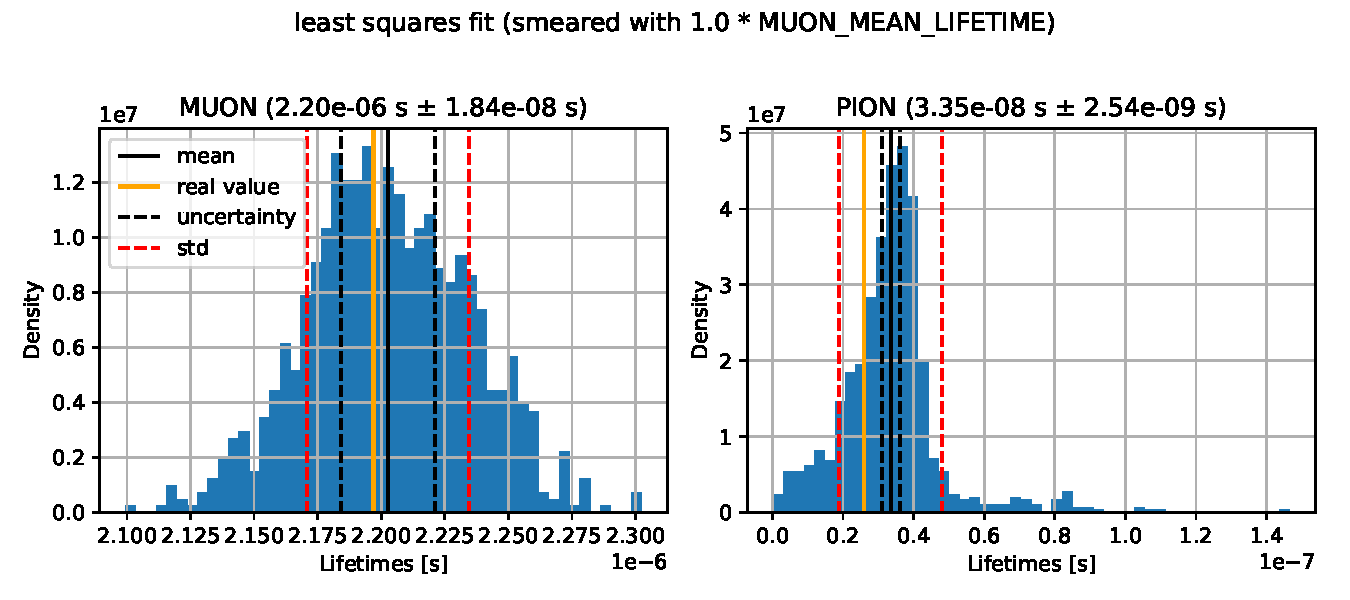
\includegraphics[width=\DoublePlotwidth\textwidth]{images/4b_hist_2_squares.pdf}
%   \caption{}
\end{subfigure}
\caption{Results of 1000 different sets of simulated and fitted data. Here the data was smeared with 1 time the \pion Mean lifetime. The MLM does not converge properly and therefore won't give usable results.}
\label{fig:results_smeared_2}
\end{figure}

\begin{figure}[h]
\begin{subfigure}{\textwidth}
  \centering
  \includegraphics[width=\Plotwidth\textwidth]{example-image-duck}
  \caption{1a}
\end{subfigure}

\begin{subfigure}{\textwidth}
  \centering
  \includegraphics[width=\Plotwidth\textwidth]{example-image-duck}
  \caption{1b}
\end{subfigure}
\caption{plots of....}
\label{fig:fig}
\end{figure}

\FloatBarrier
\section{Comparison between all results}

\begin{table}[h]
\centering
\caption{Comparison between all results and the reference value.}
\label{tab:comparison_all}
\begin{tabular}{r|r|cc}
                             & method                & muon lifetime & pion lifetime \\ \hline
reference value              &                 & \qty{2.1969811(0.0000022)e-6}{\s} & \qty{2.6033(0.0005)e-8}{\s} \\\hline
\multirow{2}{*}{no smearing} & MLM             & \qty{2.184(0.015)e-6}{\s}         & \qty{2.581(0.246)e-8}{\s}   \\
                             & LSM             & \qty{2.207(0.015)e-6}{\s}         & \qty{3.836(0.186)e-8}{\s}  \\\hline
\multirow{2}{*}{0.01 * tau}  & MLM             & \qty{2.184(0.015)e-6}{\s}         & \qty{2.581(0.246)e-8}{\s}   \\
                             & LSM             & \qty{2.184(0.015)e-6}{\s}         & \qty{2.581(0.246)e-8}{\s}   \\\hline
\multirow{2}{*}{0.1 * tau}   & MLM             & \qty{2.184(0.015)e-6}{\s}         & \qty{2.581(0.246)e-8}{\s}   \\
                             & LSM             & \qty{2.184(0.015)e-6}{\s}         & \qty{2.581(0.246)e-8}{\s}   \\\hline
\multirow{2}{*}{1 * tau}     & MLM             & \qty{2.184(0.015)e-6}{\s}         & \qty{2.581(0.246)e-8}{\s}   \\
                             & LSM             & \qty{2.184(0.015)e-6}{\s}         & \qty{2.581(0.246)e-8}{\s}    
\end{tabular}
\end{table}

\chapter{Discussion}

\chapter{Conclusion}
\section{Simple Simulation}
As discussed in section \ref{simple_simulation_results}, the MLM\footnote{binned-maximum-likelihood method} yielded much better estimations for both lifetime values when compared to LSM\footnote{least-squares method}. 

Using the pull to validate the resutls from the MLM to it self, it becomes clear, that the value for the \pion is close to the true value and the uncertainty is computed correctly. When looking at the pull for the \muon it becomes clear that there is a bias in the estimation which then also affects the accuracy of the uncertainty. 

Although the LSM is faster and more computationaly efficient, it does not yield the desired values. This is stronly visible in the estimation for the \pion as the value is way off even with the uncertainties. 

\section{A bit more Realistic}
Since the MLM yielded the better estimations in section \ref{sec:simple_simulation_results} it was to be expected, that it would also yield better results in the more accurate simulation, as seen in section \ref{sec:more_realisitic_results}.

The results of the first to smears, which $0.01 * \tau$ and $0.1 * \tau$ are close to what was achieved in the simple simulation. The MLM gives precise results close to the true value, with pull values close to what was achieved in section \ref{sec:simple_simulation_results}. 

For the case where the simulated decay times were smeared with $1 * \tau$, the MLM started to struggle as well. The problem here was, that the fitting did not converge and the algorithm just returned the initial guesses. Since the initial values were chosen quite close to the real values, this can be seen as a valid strategy by the minimization algorithm. Here the only usable values were given by the SLM values. Here the values are suprisingly close to the true values.  

\section{Comparison between the simulations}
% interpretation of the results
% compare with theory or expectations
% sources of error, limitations by the simulation

% \clearpage
% \phantomsection
% \addtocounter{chapter}{1}
% \addcontentsline{toc}{chapter}{\protect\numberline{\thechapter}{\listtablename}}
% \listoftables

% \clearpage
% \phantomsection
% \addtocounter{chapter}{1}
% \addcontentsline{toc}{chapter}{\protect\numberline{\thechapter}{\listfigurename}}
% \listoffigures

% \printbibliography[heading=bibintoc, title={Quellenverzeichnis}]
% \printbibliography[heading=bibintoc]
\IfLanguageName{ngerman}{\printbibliography[heading=bibintoc, title={Quellenverzeichnis}]}{\printbibliography[heading=bibintoc]}

\listoftables

\listoffigures

% \addtocontents{toc}{\protect\newpage}

\end{document}